\documentclass[12pt]{article}
\usepackage{amsmath,amssymb}
\usepackage{geometry}
\geometry{margin=1in}
\usepackage[hidelinks]{hyperref}
\setlength{\parindent}{0pt}
\usepackage{xcolor}
\usepackage{etoolbox}  %Supports toggle commands
\definecolor{darkblue}{RGB}{0,0,139}
\usepackage{tikz}
\usepackage{pgfplots}
\pgfplotsset{compat=1.18}
\usepackage{placeins}
\usepackage{booktabs}

%SETTINGS
\newtoggle{solutions} \togglefalse{solutions}

\begin{document}

\begin{center}
\textbf{Problem Set 4} \\
Introduction to Health Economics: EC 387 \\
Boston University \\
Spring 2026 \\
Professor Pauline Mourot
\end{center}

\vspace{1em}

\noindent \textbf{Exercise 1: TRUE/FALSE/UNCERTAIN}\\

For each of the questions below, please explain your answer.
The quality of the explanation is an important part of the grade for these problems and
can also help you earn substantial partial credit.
In answering each question, 1-3 sentences of explanation should be sufficient.

\vspace{7mm}

\noindent \textbf{QUESTION 1}\\
In the Rotschild and Stiglitz (1976) model of insurance markets with asymmetric information,
there always exist a separating equilibrium in which the low-risk consumers buy a different insurance contract than the high-risk consumers.

\iftoggle{solutions}{
{\color{darkblue}

\vspace{5mm}

FALSE.
In the Rotschild and Stiglitz (1976) model, there may not exist a separating equilibrium.
A separating equilibrium is less likely
when the low-risk population is large compared to the whole population. 
}}{}

\vspace{7mm}

\noindent \textbf{QUESTION 2}\\
The fact that health insurers try to attract healthier consumers with contract features is called ``cream skimming'',
and risk-adjustment is one way to try to prevent it.

\iftoggle{solutions}{
{\color{darkblue}

\vspace{5mm}

TRUE. Risk-adjustment is a policy tool that can be used to reduce the incentives for insurers to engage in cream skimming
by making higher-risk and low risk-consumers more equally profitable for insurers.

}}{}

\vspace{7mm}

\noindent \textbf{QUESTION 3}\\
In the Rotschild and Stiglitz (1976) model of insurance markets with asymmetric information,
the existence of high-risk consumers make the low-risk consumers worse off compared to the full information case.

\iftoggle{solutions}{
{\color{darkblue}

\vspace{5mm}

TRUE.
When the insurer cannot tell the consumer types apart,
the contract that the low-risk consumers would buy in the perfect information case would attract high-risk consumers, so the insurer would not offer that contract.
When a separating equilbrium exists,
the insurer would offer a contract that is more expensive and less generous than the one the low-risk consumers would buy in the perfect information case.
This contract lies on a lower indifference curve compared to the full information contract,
so the low-risk consumers are worse off than in the full information case.

\newpage

}}{}

\vspace{7mm}

\noindent \textbf{QUESTION 4}\\
Though adverse selection could shape contract features offered by insurers like plan generosity or coverage for certain medical procedures or coverage in theory,
there is no empirical evidence that health insurers respond to such selection incentives.

\iftoggle{solutions}{
{\color{darkblue}

\vspace{5mm}

FALSE. We saw in class the research by Geruso, Layton and Prinz (2019) which
showed that health insurers responded to selection incentives by making drug formularies more restrictive in the ACA Marketplace plans compared to self-insured employers' plans
when the drugs are used by less profitable patients.

}}{}


\vspace{7mm}

\noindent \textbf{QUESTION 5}\\
Even though health insurance can increase healthcare utilization and spending,
it may have beneficial impacts on enrollees beyond healthcare utilization that may make it valuable for society.

\iftoggle{solutions}{
{\color{darkblue}

\vspace{5mm}

TRUE. Can discuss the research on financial health or on health directly looking at mortality or preventive care for example.
}}{}

\vspace{7mm}

\noindent \textbf{QUESTION 6}\\
Risk-adjustment may give incentives for insurers to ``game'' the system to receive higher payments for their enrollees.

\iftoggle{solutions}{
{\color{darkblue}

\vspace{5mm}

TRUE. Because risk-adjustment is based on diagnosis codes,
and diagnosis codes could be manipulated,
insurers may have incentives to encourage doctors to code more ``profitable'' diagnoses for their enrollees to receive higher payments.
This is the research from Geruso and Layton (2020) that we mentionned in class.
}}{}

\vspace{7mm}

\iftoggle{solutions}{}{\newpage}



\noindent \textbf{Exercise 2: Impact of a mandate on a selection market}\\

\medskip

Assume that there are 50 individuals who are considering buying health insurance from a monopolist insurer.
Each individual faces a probability $p$ of needing to go to the hospital.
Person 1 has a probability of hospitalization of $0.50$ (i.e., a $50/50$ chance);
Person 2 has a probability of $0.49$;
Person 3 has a probability of $0.48$;
Person 4 has a probability of $0.47$;
\ldots;
and Person 50 has probability $0.01$ (i.e., a $1\%$ chance).

\medskip

Other than these differences in probabilities, all of the individuals are otherwise identical:
they have identical income levels when healthy (income $y=\$50{,}000$),
and when they get sick they face identical medical costs of $h=\$30{,}000$.

\medskip

Without any health insurance, each individual has expected utility given by
\[
EU(p)=p\sqrt{y-h}+(1-p)\sqrt{y}.
\]
, so the utility is such that $u(c) = \sqrt{c}$.
\medskip

A monopolist health insurer offers a full insurance contract to these 50 individuals
(i.e., no deductible, no coinsurance).

\bigskip
\noindent\textbf{a.} Calculate the marginal cost curve facing the insurer and graph it
(i.e., the horizontal axis is the number of individuals buying insurance ranging from $Q=1$ to $Q=50$,
and the vertical axis is the firm's marginal cost). Label the curve carefully.

\medskip
\textit{Hint: In this problem, the first individual buying insurance will have the highest probability of a hospitalization,
and the last person buying will have the lowest probability.}\\
\textit{Hint 2: The insurer's marginal cost is the expected medical cost of the marginal enrollee, i.e. the additional enrollee buying insurance.}\\
\textit{Hint 3: Notice that the expected medical costs decrease along a line, and round the intercept and slope to the nearest integer.}

\iftoggle{solutions}{
{\color{darkblue}

\medskip

Under full insurance, the insurer's marginal cost is the expected medical cost of the marginal enrollee.
This means the marginal cost curve will be equal to the expected cost of each new enrollee.
The first person to buy insurance is Person 1, who has a probability of hospitalization of $0.50$.\\
The expected medical cost of Person 1 is $0.50 \cdot \$30{,}000 = \$15{,}000$.\\
The second person to buy insurance is Person 2, who has a probability of hospitalization of $0.49$.\\
The expected medical cost of Person 2 is $0.49 \cdot \$30{,}000 = \$14{,}700$.\\
Continue the logic to the 50th person, who has a probability of hospitalization of $0.01$.\\
The expected medical cost of Person 50 is $0.01 \cdot \$30{,}000 = \$300$.\\

\vspace{2mm}

It looks like a line that decreases with \$300 increments.
This is a downward-sloping line that starts at $MC(1)=15000$ and ends at $MC(50)=300$.\\

\vspace{2mm}

To get the equation of the line, we know that $MC(Q) = a + b Q$ where $a$ and $b$ are the intercept and slope of the line, respectively.
Using the two points $(1, 15000)$ and $(50, 300)$, we can solve for $a$ and $b$:
\begin{align*}
15000 &= a + b \cdot 1 \\
300 &= a + b \cdot 50
\end{align*}

Subtract the first line from the second to get
\begin{align*}
300 - 15000 &= (a + b \cdot 50) - (a + b \cdot 1) \\
-14700 &= b \cdot 49 \\
b &= \frac{-14700}{49} \approx -300
\end{align*}

Then plug $b$ back into the first line to get
\begin{align*}
15{,}000 &= a - 300 \cdot 1 \\
a &= 15{,}000 + 300 = 15{,}300
\end{align*}    

Therefore, the marginal cost curve is
\begin{align*}
    MC(Q) = 15{,}300 - 300Q.
\end{align*}

See graph below.

}}{}

\bigskip
\noindent\textbf{b.} Calculate the average cost ($AC$) curve given the marginal cost curve assuming that there are no fixed costs for the insurer.

\medskip
\textit{Hint: use the marginal cost curve equation you found in a) to get the total cost curve,
which you can then use to get the average cost curve as we saw in class.}


\iftoggle{solutions}{
{\color{darkblue}

\medskip


As we saw in class and following the hint, the total cost curve can be obtained by integrating the marginal cost curve:
\begin{align*}
TC(Q) &= \int MC(Q) dQ \\
        &= \int (15{,}300 - 300Q) dQ \\
        &= 15{,}300Q - 150Q^2,
\end{align*}

Then we know that the average cost curve is the total cost divided by $Q$:
\begin{align*}
AC(Q) &= \frac{TC(Q)}{Q} \\
&= \frac{15{,}300Q - 150Q^2}{Q} \\
&= 15{,}300 - 150Q.
\end{align*}

\textit{Note: Some of you may not have used the hint and computed the average cost at each point and noticed it was a straightline too.
This would give you a similar answer but a different intercept such that $AC(Q) = 15{,}150 - 150Q$.
This is also correct, and the difference in intercepts is not important for the rest of the problem.
You would get full marks in that case too.}
}}{}

\bigskip
\noindent\textbf{c.} Is the $MC$ curve above or below the $AC$ curve at $Q>1$?
Provide economic intuition in 1--3 sentences.

\iftoggle{solutions}{
{\color{darkblue}

\medskip

For $Q>1$, the marginal cost curve is below the average cost curve.
You can easily see this by plotting both curves on the same graph (see graph below), or by plugging in any value of $Q$ greater than 1 into the two equations.
}}{}

\bigskip
\noindent\textbf{d.} Next, calculate the demand curve facing the firm and graph the demand curve.
Again, label this demand curve and graph it alongside the $MC$ and $AC$ curves.

\medskip
\textit{Hint: Here is one way to approach this problem, although you can solve the problem any way you would like.
Start with a table with each value of $p$ between $0.5$ and $0.01$ and compute the certainty equivalent ($CE$) at each value of $p$.
Next, use this to compute the risk premium as a function of $p$.
The demand curve can then be derived as the willingness to pay ($WTP$), which is the sum of the $MC$ and the risk premium;
i.e., $WTP = MC + RP$ at each value of $p$.}

\iftoggle{solutions}{
{\color{darkblue}

\medskip

Using the hint, we can compute the certainty equivalent for each individual (at each $p$),
then recover the risk-premium (RP) as the difference between the expected gain and
the certainty equivalent at each $p$,
and finally get the willingness to pay (WTP) as the sum of the marginal cost and the risk premium.

\vspace{3mm}

\textbf{Step 1: Certainty equivalent}\\
It is the amount the consumer would be willing to accept to avoid the gamble,
i.e. such that the expected utility from the gamble (here, no insurance) is equal to the utility of the certainty equivalent.
Denote the certainty equivalent $CE_i$ for individual $i$.
It is the solution to the following equation:
\begin{align*}
EU(\text{no insurance}_{i}) &= u(CE_i) \\
p_i\sqrt{y-h}+(1-p_i)\sqrt{y} &= \sqrt{CE_i} \\
p_i\sqrt{50{,}000-30,000}+(1-p_i)\sqrt{50{,}000} &= \sqrt{CE_i} \\
CE_i &= \left(p_i\sqrt{20{,}000}+(1-p_i)\sqrt{50{,}000}\right)^2
\end{align*}
You can compute this for each value of $p_i$ (see solutions in Excel file).

\vspace{3mm}

\textbf{Step 2: Risk premium}\\
The risk premium is the difference between the expected income $Y$ \textit{without insurance} and the certainty equivalent:
\begin{align*}
RP_i &= E[\text{no insurance}_i] - CE_i \\
&= (p_i \cdot (50{,}000-30{,}000) + (1-p_i) \cdot 50{,}000) - CE_i
\end{align*}
Once again, you can compute this for each value of $p_i$ (see solutions in Excel file).

\vspace{3mm}

\textbf{Step 3: Willingness to pay}\\
The willingness to pay for insurance is the sum of the marginal cost and the risk premium:
\begin{align*}
WTP_i &= MC_i + RP_i
\end{align*}

See the companion Excel file for the exact solutions.

}}{}

\bigskip
\noindent\textbf{e.} Is the demand curve above or below the $MC$ curve at $Q=1$?
What about at $Q=50$?
Provide economic intuition for both answers in 1--3 sentences.

\iftoggle{solutions}{
{\color{darkblue}

\medskip

Using your calculations from the previous question,
the demand curve is above the $MC$ curve at both $Q=1$ and $Q=50$.
This makes sense because all consumers are risk averse, so they are willing to pay a positive risk premium above the expected medical costs (which is the marginal cost) to get insurance.
The demand curve is much higher than the $MC$ curve at $Q=1$ because the first consumer to buy insurance is the one with the highest probability of hospitalization, and therefore the highest risk premium.
}}{}

\bigskip
\noindent\textbf{f.} Next, calculate the profit-maximizing choice for the monopolist and label this point on the figure from part (d).
(When your calculations imply a non-integer number of consumers, round to the nearest integer.
For example, 5.3 is rounded to 5 and 5.7 is rounded to 6.
Round values like 5.5 to 6.)

\medskip
\textit{Hint: The profit-maximizing choice for the monopolist requires calculating the marginal revenue ($MR$) curve.
You can work with the following linear inverse demand curve,
which is a fairly accurate linear approximation of the true inverse demand curve:}
\[
P = 17{,}500 - 333 Q.
\]
\textit{From this linear inverse demand curve, you can calculate the $MR$ curve and solve for the optimal profit-maximizing choice
assuming linear demand following the formulas in the lecture slides and the $MC$ curve from above.}

\iftoggle{solutions}{
{\color{darkblue}

\medskip

Using the linear approximation,
\[
P(Q)=17{,}500 - 333Q.
\]
Total revenue is
\[
TR(Q)=P(Q)\cdot Q=(17{,}500 - 333Q)Q,
\]
so marginal revenue is
\[
MR(Q)=17{,}500 - 666Q.
\]

The optimal quantity $Q^*$ is the one that equates marginal revenue and marginal cost:
Set $MR(Q^*)=MC(Q^*)$:
\begin{align*}
17{,}500 - 666Q^* &= 15{,}300 - 300Q^* \\
\end{align*}
This gives
\begin{align*}
17{,}500 - 15{,}300 &= 666Q^* - 300Q^* \\
2{,}200 &= 366Q^* \\
Q^* &\approx 6.01.
\end{align*}

So the monopolist insures about $6$ individuals.
Using the linear demand approximation, the corresponding price is
\begin{align*}
P^* &= 17{,}500 - 333 \cdot 6.01 \\
&\approx 15{,}500.
\end{align*}

So the monopolist sells insurance only to the sickest 6 consumers at price \$15,500.

\vspace{2mm}

\textit{Note: we also accept answers that would have noticed that 
$MR - MC$ in the Excel file is positive at $Q=6$ and negative at $Q=7$, so the profit-maximizing choice is between 6 and 7,
which means that the monopolist sells insurance to about 6 individuals.
See the companion Excel file for the exact solutions.}

\begin{figure}
    \centering
    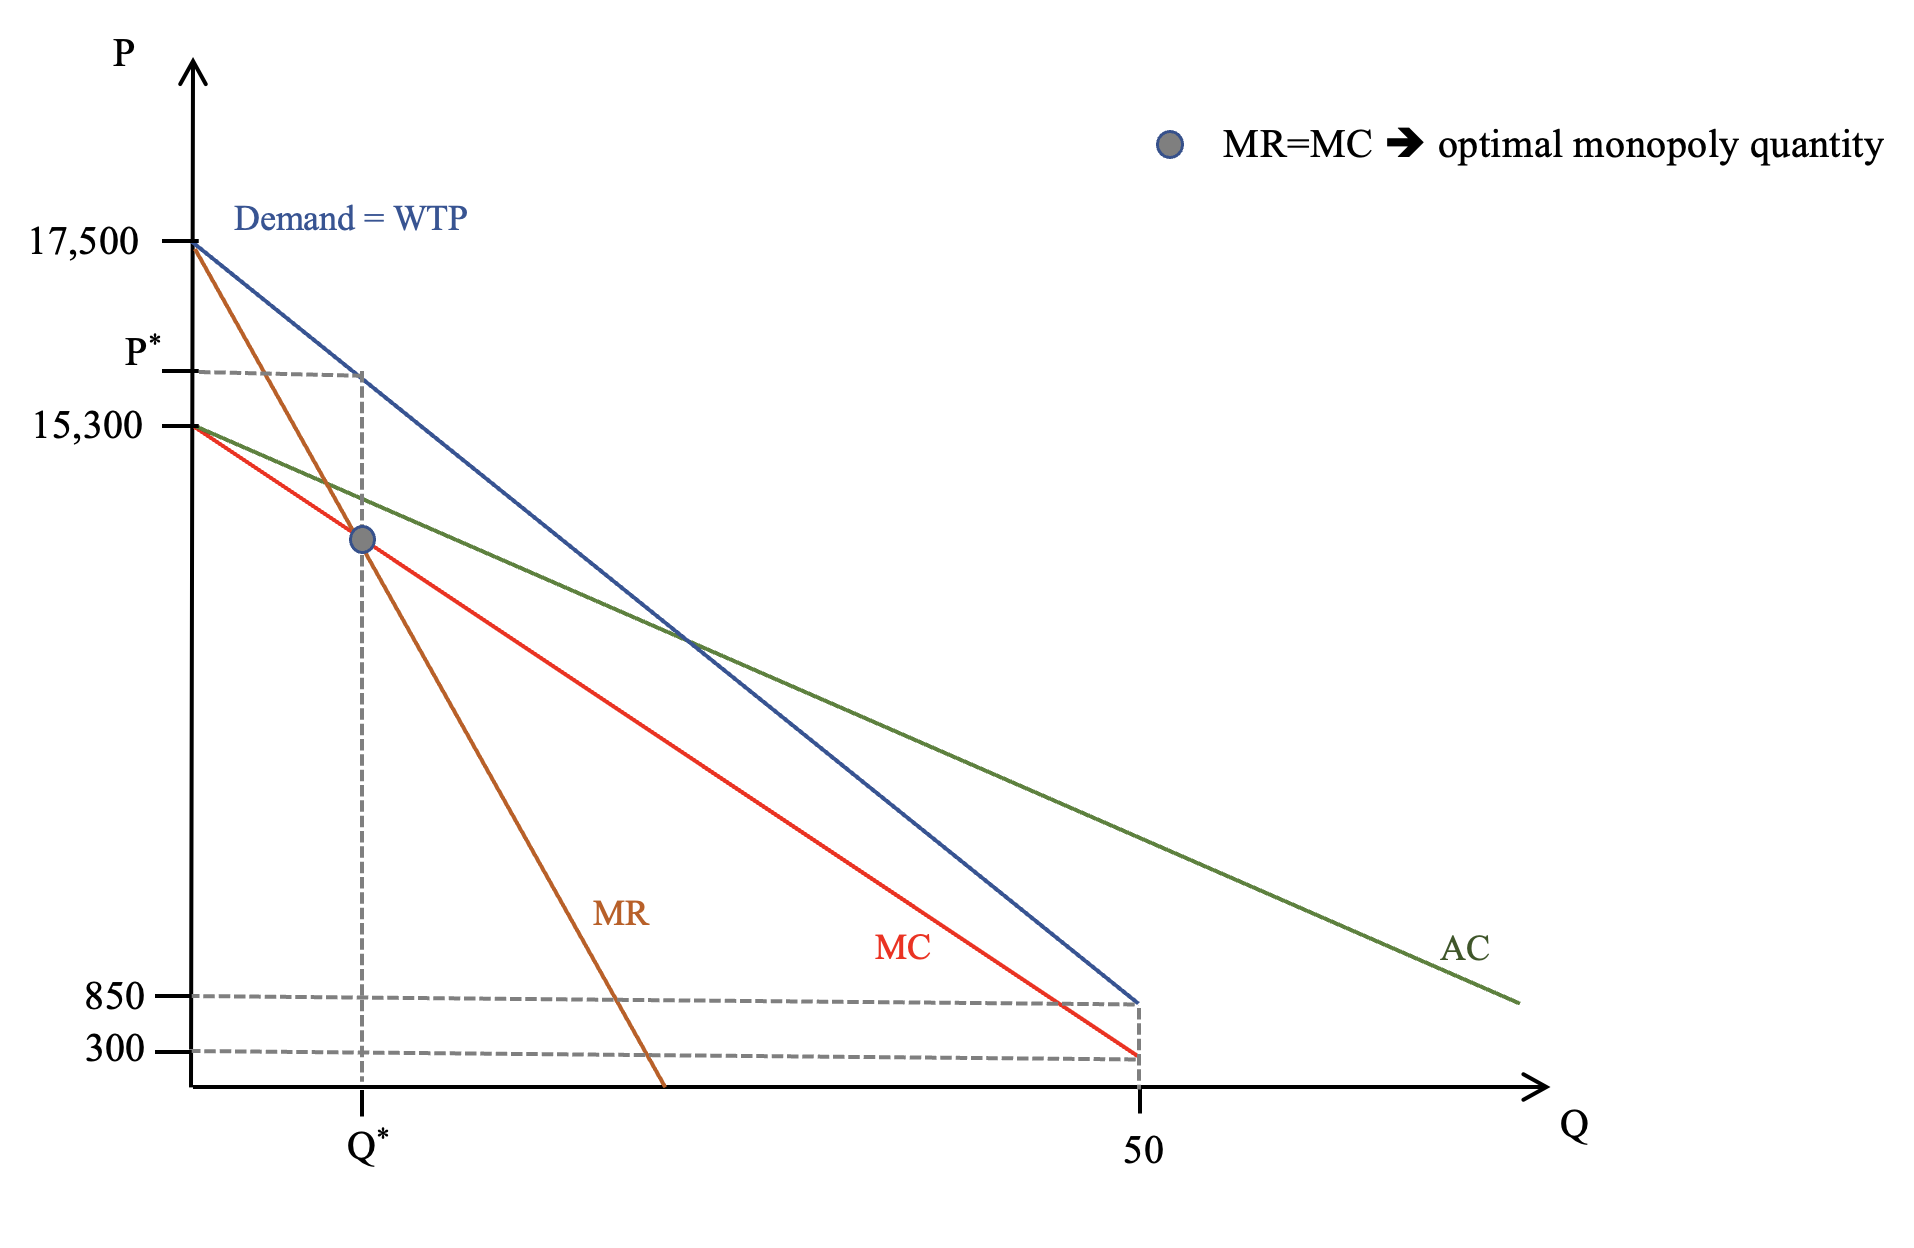
\includegraphics[width=0.7\textwidth]{material_PS4/PS4_g1.png}
\end{figure}

\FloatBarrier
}}{}

\bigskip
\noindent\textbf{g.} Is there any adverse selection in the market,
according to your answer to part (f)?
If there is adverse selection,
does the market completely unravel or does it only partially unravel?
If there is adverse selection,
does it affect the relatively healthy or relatively sick, according to this model?
Provide economic intuition in 1-3 sentences for why this is the case in this model.
\iftoggle{solutions}{
{\color{darkblue}

\medskip

Yes, there exist adverse selection on this market:
the MC curve is decreasing and the riskiest consumers
are the ones who buy first with the highest willingness to pay.
This market partially unravels:
some consumers (6) will get insurance while the rest (44) will remain uninsured
while they would be willing to buy insurance (positive risk-premium).
The relatively healthy consumers will end up not buying insurance in equilibrium here,
because the premium offered is too high for them,
since the sickest consumers buy insurance first.
}}{}

\bigskip
\noindent\textbf{h.} Compute the consumer surplus in part (f).

\iftoggle{solutions}{
{\color{darkblue}

\medskip

The consumer surplus is the triangle area below the demand curve at the equilibrium price and quantity.
Reminder: the area of a triangle is $\frac{1}{2} \cdot \text{base} \cdot \text{height}$.
It is equal to 
\begin{align*}
    A &= \frac{1}{2} \cdot (WTP^{MAX} - P^*) \cdot Q^*\\
    &= \frac{1}{2} \cdot (17{,}500 - 15{,}500) \cdot 6 \\
    &= 6{,}000
\end{align*}

\textit{Note: You could also sum the difference between the willingness to pay and
the price for each of the 6 consumers who buy insurance in the Excel file
to get the consumer surplus.
It is equal to something closer to \$5{,}000 because of approximation,
which does not matter for the purpose of this problem.
See companion Excel file for the exact solutions.}

\vspace{3mm}

\begin{figure}
    \centering
    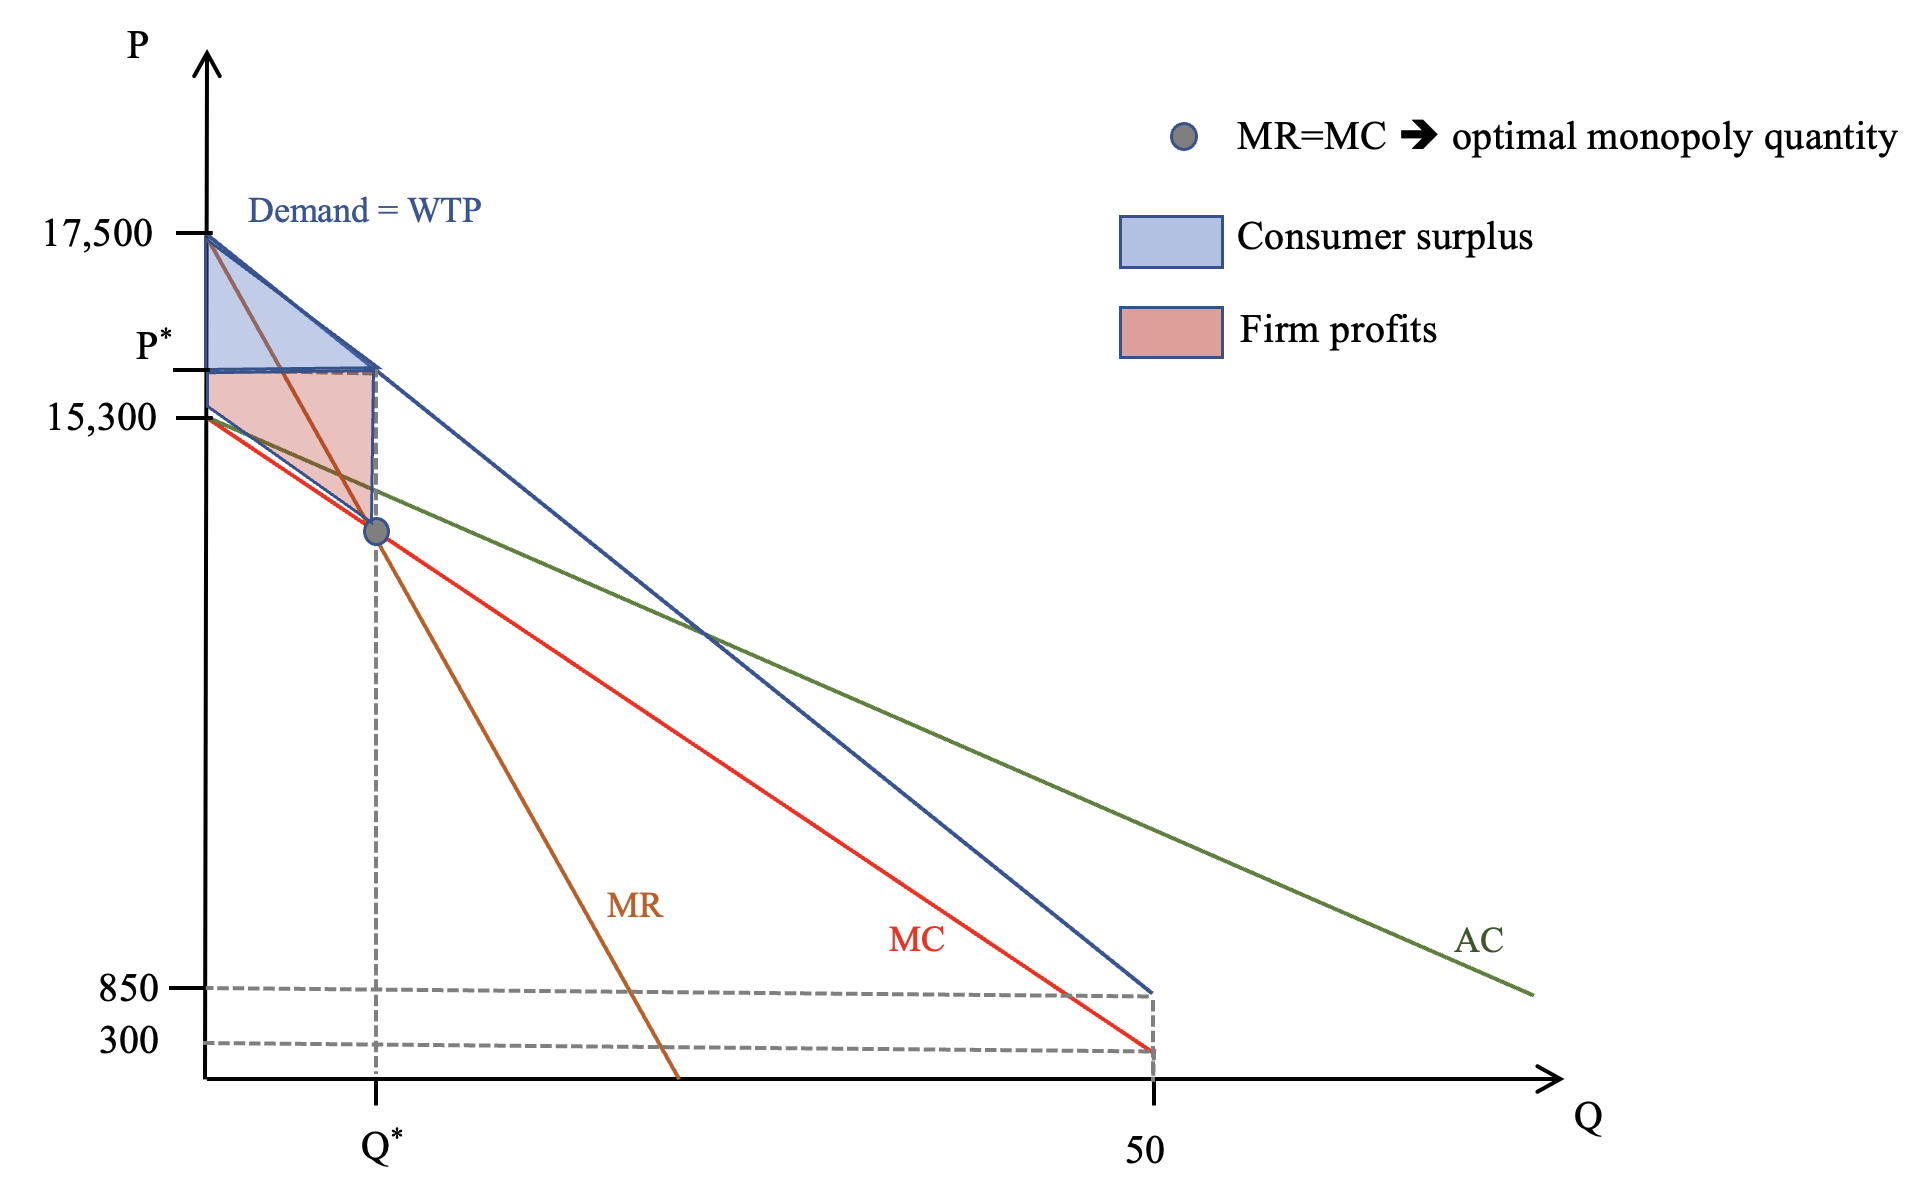
\includegraphics[width=0.7\textwidth]{material_PS4/PS4_g3.png}
\end{figure}
(The graph includes firms' profits but this wasn't needed in your answer to this question.)

\FloatBarrier

}}{}

\bigskip
\noindent\textbf{i.} Suppose that the government passes a mandate that everyone must purchase health insurance,
and the government also imposes a price ceiling of $\$8{,}000$ on the monopolist insurer selling the insurance plan.
Graphically indicate the new consumer surplus as a result of this policy.
Calculate the new firm profits.
Are firms still earning profits?
Explain intuitively in 1--3 sentences.
Are any individuals helped by the combination of the individual mandate and the price ceiling?
Are any individuals harmed?
(When your calculation imply a non-integer number of consumers, round to the nearest integer. For example, 5.3 is rounded to 5 and 5.7 is rounded to 6.
Round values like 5.5 to 6.)

\medskip

\textit{Hint: Use the approximation of the demand given in a hint above as $P = 17{,}500 - 333 Q$.}

\iftoggle{solutions}{
{\color{darkblue}

\medskip

Now, the firm will price at the maximum price of \$8,000 and sell insurance to all 50 individuals.

\vspace{2mm}

\textbf{Consumer surplus.}\\
Draw the graph to help you visualize the change in consumer surplus (see below).

\FloatBarrier

\begin{figure}[htbp]
    \centering
    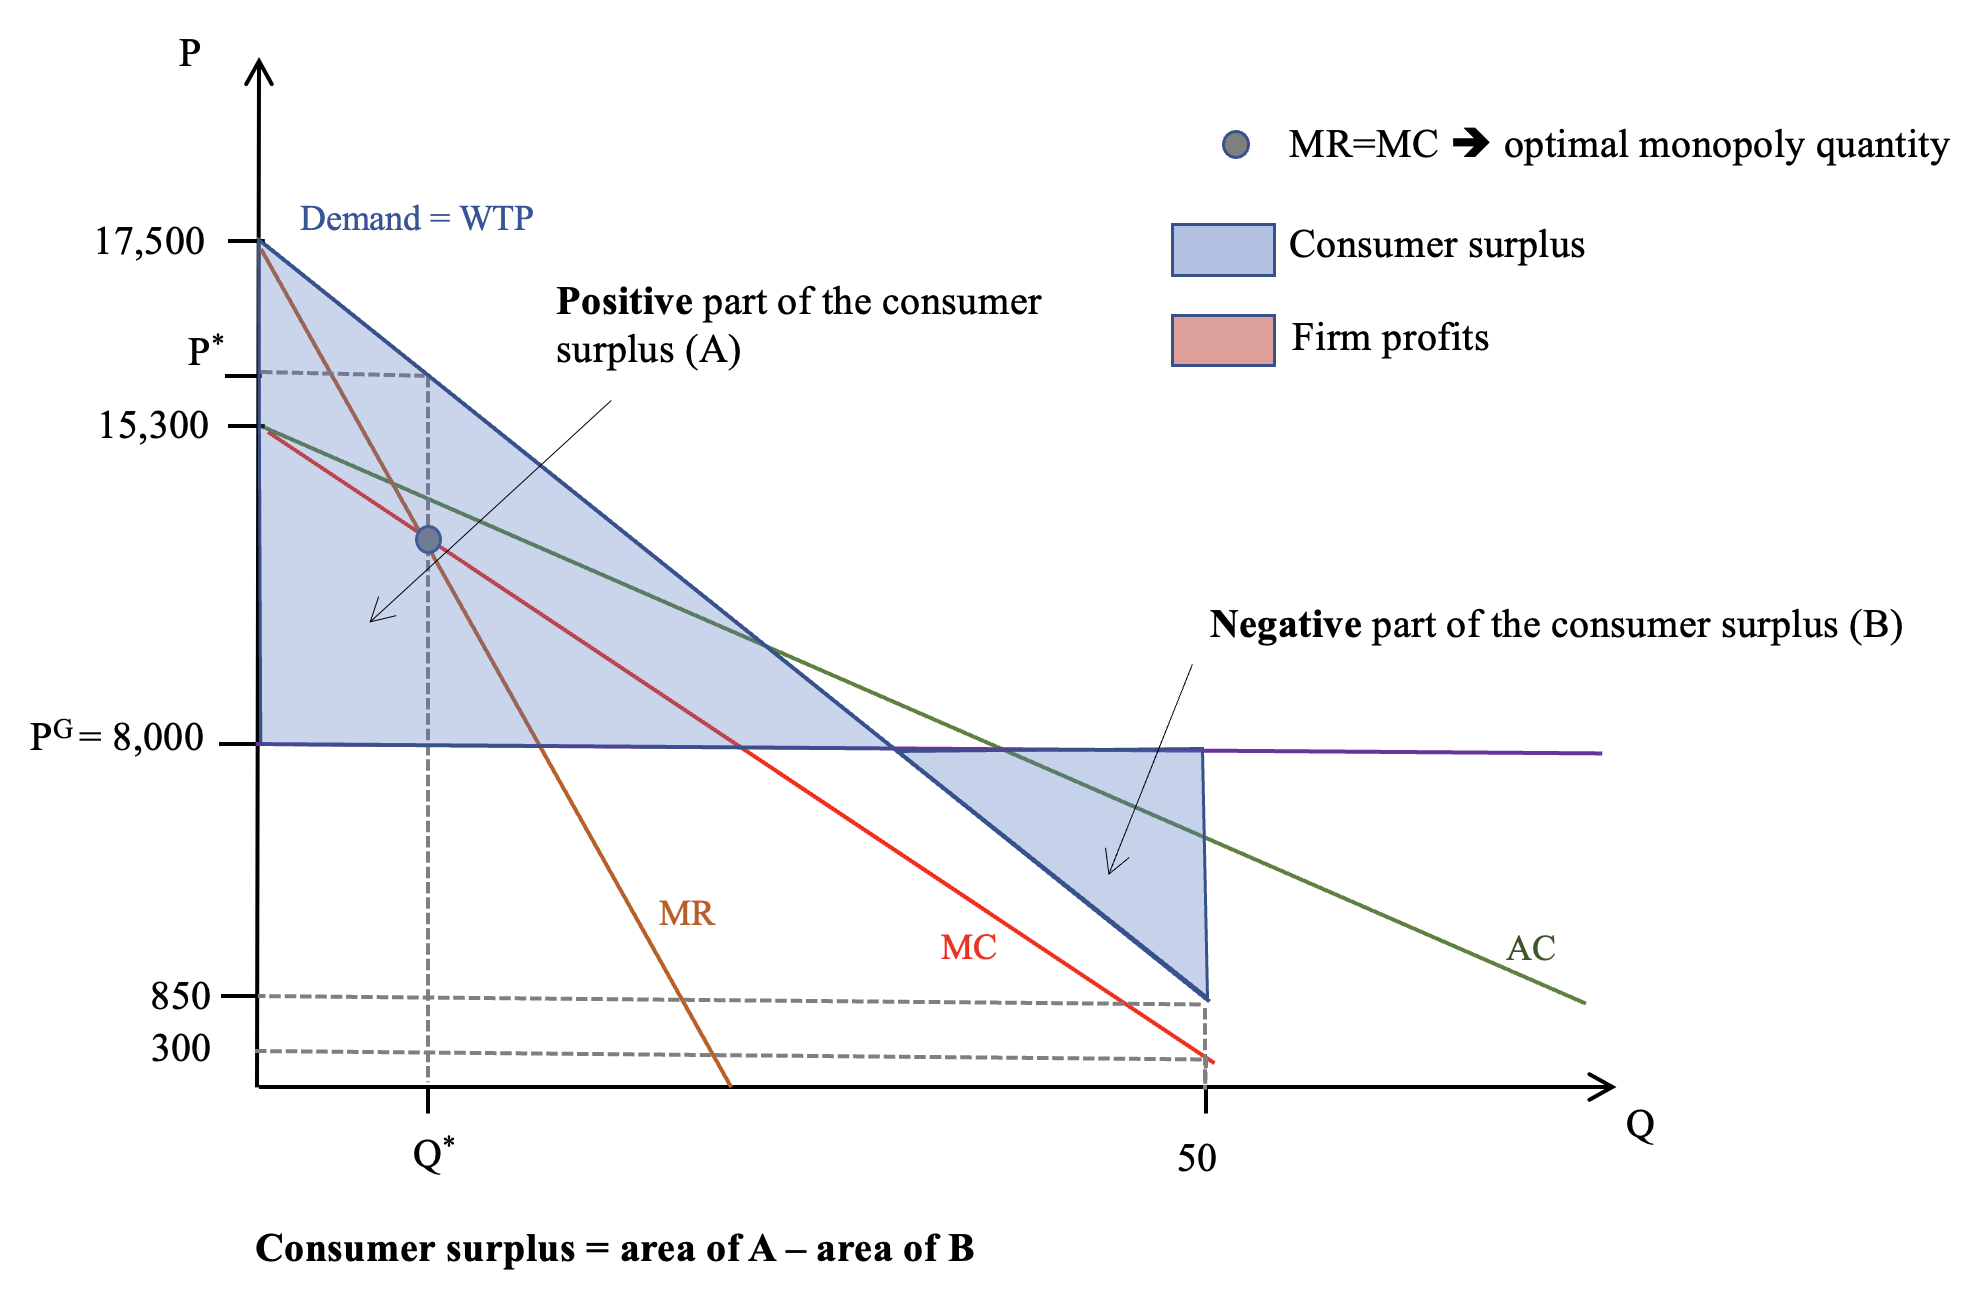
\includegraphics[width=0.7\textwidth]{material_PS4/PS4_g4.png}
\end{figure}

First, note that not all consumers have a demand (WTP) above \$8,000,
so only some of the consumers will benefit from the policy.
You can find the number of consumers with WTP above \$8,000 by looking at the Excel file
or by solving for $Q$ in the demand curve equation when $P=8{,}000$:
\begin{align*}
8{,}000 &= 17{,}500 - 333Q \\
333Q &= 9{,}500 \\
Q &\approx 28.52
\end{align*}
Rounding up to the nearest integer, we find that 29 consumers will benefit
while the remaining 21 consumers will be harmed by the policy.

The consumer surplus for the 29 consumers who benefit from the policy
is the area of the triangle between the demand curve and the price ceiling (A), which is
\begin{align*}
    A &= \frac{1}{2} \cdot (WTP^{MAX} - 8{,}000) \cdot 29 \\
    &= \frac{1}{2} \cdot (17{,}500 - 8{,}000) \cdot 29 \\
    &\approx 137,750
\end{align*}

The consumer surplus for the 21 consumers who are harmed by the policy
is the area of the triangle between the demand curve and the price ceiling (B), which is
\begin{align*}
    B &= -\frac{1}{2} \cdot (8{,}000 - WTP^{MIN}) \cdot 21 \\
    &= -\frac{1}{2} \cdot (8{,}000 - (17{,}500 - 333 \cdot 50)) \cdot 21 \\
    &=-75,075
\end{align*}

Note that B is negative because the price is above their willingness to pay (i.e. above their demand),
so they are harmed by the policy.

The total consumer surplus is the sum of the two:
\begin{align*}
    CS &= A + B \\
    &\approx 137,750 - 75,075 \\
    &\approx 62,675
\end{align*}
The total consumer surplus is positive under this policy.
The first 29 consumers have a positive consumer surplus with the policy,
while the remaining 21 consumers are harmed by the policy.

\vspace{2mm}

\textit{Note: you can also caculate consumer surplus by substracting each consumer WTP
from the mandate price in the Excel file and sum across individuals.
See attached Excel solution.}

\vspace{2mm}

\textbf{Firm profits.}
The firm has to sell to everyone at a price of \$8,000.
Based on the graph below, it will loose money on the first $X$ consumers,
because the mandate price is below the marginal cost for these consumers,
but earn profit on the remaining $50-X$ consumers for whom the marginal cost is below the mandate price.
\begin{figure}[htbp]
    \centering
    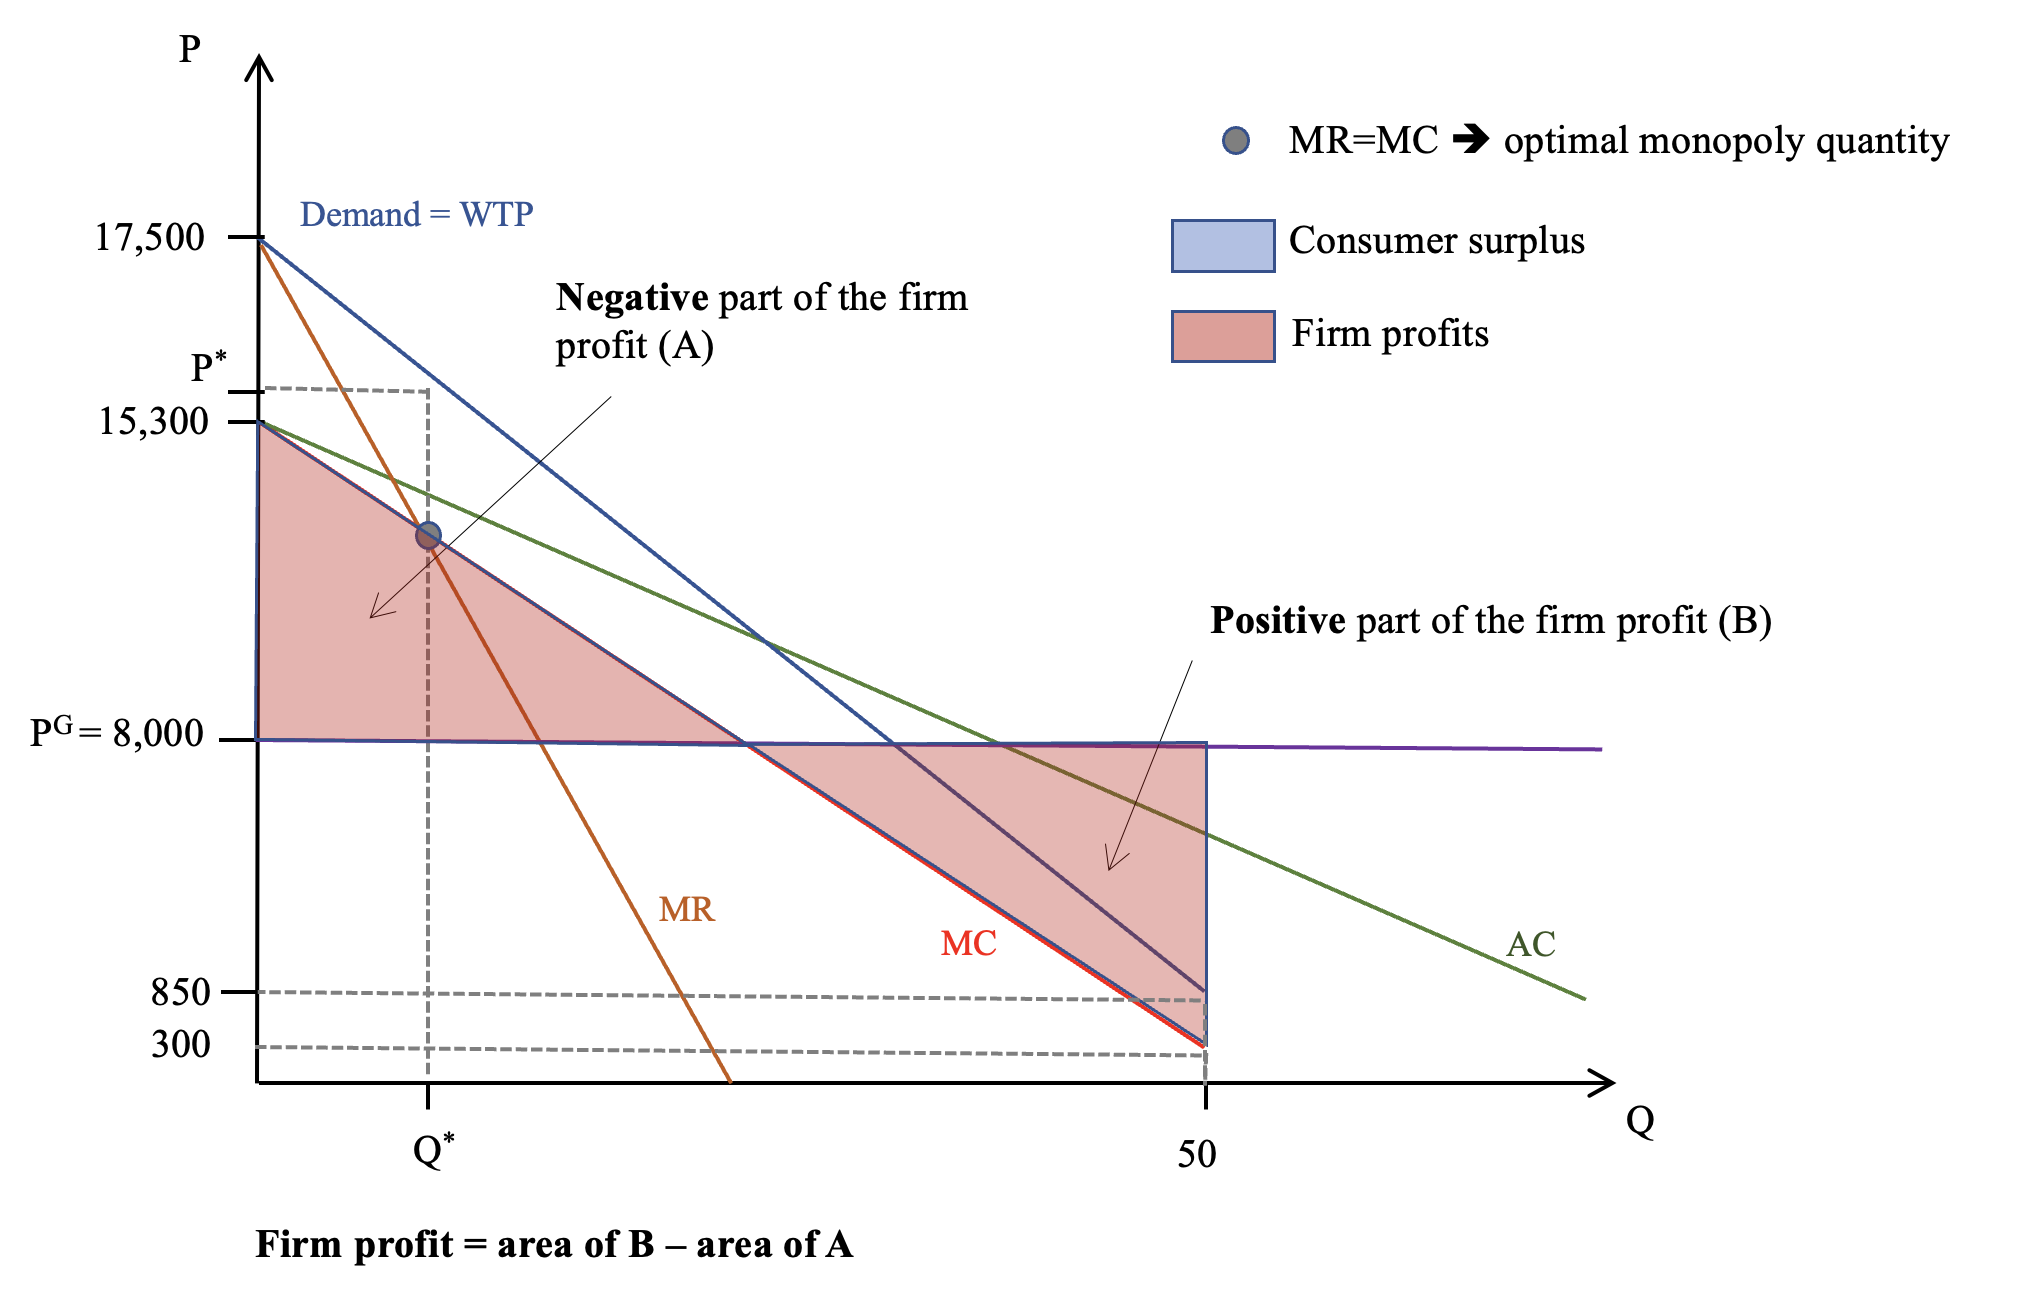
\includegraphics[width=0.7\textwidth]{material_PS4/PS4_g5.png}
\end{figure}
\FloatBarrier

What is $X$?
It is the point where the marginal cost curve intersects the price ceiling:
\begin{align*}
8{,}000 &= 15{,}300 - 300X \\
300X &= 15{,}300 - 8{,}000 \\
300X &= 7{,}300 \\
X &\approx 24.3
\end{align*}
Rounding up to the nearest integer, we find that the firm will lose money on the first
24 consumers and earn profit on the remaining 26 consumers.

The total profit is the sum of the profits from each consumer:
\begin{align*}
    \pi &= -\frac{1}{2} \cdot (15{,}300 - 8{,}000) \cdot 24 + \frac{1}{2} \cdot (8{,}000 - (15{,}300 - 300 \cdot 50)) \cdot 26 \\
    &\approx -87,600 + 100,100 \\
    &\approx 12,500
\end{align*}
The firm is still earning profits under this policy.
It looses money on the first 24 consumers but earns more money on the remaining 26 consumers,
and the profits it makes on the healthy consumers is enough to compensate for the loss 
on the first 24 consumers.
}}{}

\bigskip
\noindent\textbf{j.} Using concepts from the class as well as your own knowledge, thoughts, and opinions,
describe the strengths and limitations of the answers to part (j) as an economic evaluation of the individual mandate component of the Affordable Care Act.
Limit your answer to 500 words.

\iftoggle{solutions}{
{\color{darkblue}

\medskip

The individual mandate in part i) allows for the monopolist to still earn positive profits
in the presence of a low price ceiling.
Without the mandate, but with the price ceiling,
the monopolist would make negative profits,
so the monopolist would exit without the individual mandate.
The individual mandate guarantees the participation of health insurers
in the market despite a price ceiling.

\vspace{2mm}

Furthermore, the individual mandate forces healthy individuals to buy insurance
even when the price of insurance is higher than their willingness-to-pay.
Note that in the absence of price ceiling but with an individual mandate,
a monopolist would have incentives to raise its price infinitely,
so the individual mandate needs to be coupled with a price ceiling
if there is a monopoly in the insurance market. 
The combination of price ceiling and individual mandate allows for
redistribution from healthy to sick individuals.
Additionally, health insurers can also get higher profits
(depending on the price ceiling level), hence also implying
redistribution from healthy individuals to insurers.

\vspace{2mm}

Overall, the benefits and limitations of the mandate depend on the weight
society puts on protecting sicker individuals at the expense of the healthy.
The benefits and limitations also crucially depend on how low or high
the price ceiling is compared to the distribution of willingness-to-pay
in the society.

}}{}


\vspace{10mm}

\noindent \textbf{Exercise 3: Risk adjustment and cream skimming}

\medskip

You are a VP at Anthem Health Insurance Company.
You are in charge of strategic thinking for Anthem's private Medicare plans.
You set the price for the plan and you set the schedule of benefits,
such as doctor networks, copays, and so on.
Regulations require Anthem to enroll any Medicare-eligible person who wants to join the plan,
and you cannot price discriminate.

\vspace{2mm}

In addition to the premium you collect (typically between \$0 and \$100 per month),
the government gives a subsidy of \$500 per month per enrollee. Therefore,

\begin{equation*}
\text{Profits} = \text{premiums} + \text{subsidy} - \text{costs}.
\end{equation*}

You are competing against several other insurers in most markets.

\bigskip
\noindent\textbf{a.} Based on what we discussed in class,
discuss which strategies you could want to put in place to maximize profits,
and give examples on how you would implement them.

\iftoggle{solutions}{
{\color{darkblue}

\medskip

You would want to engage in ``cream-skimming'' by trying to attract healthier enrollees
who are less costly to insure and/or by trying to avoid enrolling sicker enrollees
who are more costly to insure.
For example:
\begin{itemize}
    \item[-] Poor coverage for hospitals that sicker patients value (hospitals with very good cancer care for example)
    \item[-] Make it hard to access high-cost care so that consumers who need high-cost care would want to avoid your plan
    \item[-] Make primary care visits almost free while specialist care would be poorly covered
    \item[-] Do not cover drugs and procedures that are used by sicker patients
    \item[-] Offer free gym memberships
    \item[-] Advertise the plan in places where healthier people are more likely to be (e.g., gyms, zip codes with higher-income people, etc.)
    \item[] \dots
\end{itemize}

}}{}

The government is changing its payment formula. It now adjusts its subsidy so that it attempts to exactly balance costs. It does this by adjusting the subsidy as a function of demographics and diagnoses. Diagnoses are given by diagnosis codes that are reported in medical claims (bills) sent from the doctors to the insurance company.

The new subsidy formula for consumer $i$ is

\begin{equation*}
\text{Subsidy}_i = 500 \times \text{Risk\_score}_i.
\end{equation*}

where

\begin{align*}
\text{Risk\_score}_i 
= \sum_j \text{Coefficient}_j \cdot 
\mathbf{1}\big[\text{Diagnosis or Demographic Characteristic } j\big].
\end{align*}
with $j$ indexing the covered diagnoses and demographic characteristics.\\
(Reminder: $\mathbf{1}[\cdot]$ is the indicator function that takes value 1
if the patient has the specific diagnosis or demographic characteristic, and 0 otherwise.)

\vspace{2mm}

Here are the coefficients for the covered diagnoses and demographic characteristics:
\begin{center}
\begin{tabular}{l c}
\toprule
\textbf{Demographic Characteristic} & \textbf{Coefficient} \\
\midrule
Male (65--80) & 0.50 \\
Male (over 80) & 1.50 \\
Female (65--80) & 0.25 \\
Female (over 80) & 1.00 \\
\midrule
\textbf{Diagnosis} & \textbf{Coefficient} \\
\midrule
Diabetes & 1.75 \\
Cancer & 3.00 \\
Heart Disease & 0.50 \\
Multiple Sclerosis & 4.50 \\
\bottomrule
\end{tabular}
\end{center}

\bigskip
\noindent\textbf{b.} Use the table above to determine the monthly subsidy amount for the following three patients.

\begin{itemize}
\item[-] Patient 1: Female age 70 with diabetes.
\item[-] Patient 2: Male age 86 with Multiple Sclerosis and Cancer.
\item[-] Patient 3: Female age 65 with no diagnosed conditions.
\end{itemize}

\iftoggle{solutions}{
{\color{darkblue}

\medskip

\begin{itemize}
\item[-] Patient 1: Female age 70 with diabetes.
\begin{align*}
    \text{subsidy} &= 500 \times (0.25 + 1.75) \\
                &= 500 \times 2.00 \\
                &= 1{,}000
\end{align*}
\item[-] Patient 2: Male age 86 with Multiple Sclerosis and Cancer.
\begin{align*}
    \text{subsidy} &= 500 \times (1.50 + 4.50 + 3.00) \\
                &= 500 \times 9.00 \\
                &= 4{,}500
\end{align*}
\item[-] Patient 3: Female age 65 with no diagnosed conditions.
\begin{align*}
    \text{subsidy} &= 500 \times 0.25 \\
                &= 125
\end{align*}
\end{itemize}

}}{}

\bigskip

\noindent\textbf{c.} Assume that risk adjustment works perfectly in its intended purpose.
In that case, which person of the three (if any) would be the most profitable to Anthem?

\iftoggle{solutions}{
{\color{darkblue}

\vspace{7mm}

If risk-adjustment works perfectly,
then the subsidy would exactly balance the costs of insuring each patient.
In that case, all three patients would be equally profitable to Anthem \textit{in expectation}.

}}{}

\bigskip

\noindent\textbf{d.} What would happen if Anthem decides to provide excellent coverage for high-quality expensive care?

\iftoggle{solutions}{
{\color{darkblue}

\vspace{7mm}

If Anthem provides high-quality expensive care coverage,
higher-risk consumers would be more likely to enroll in Anthem's plan
because the plan is more attractive to them
(they value high-quality for expensive care more since more likely to need it).
However, because of risk-adjustment,
Anthem would receive higher government payments for these sicker enrollees.
Overall, Anthem may find it profitable to provide high-quality expensive care
because government payments can compensate for the higher costs of attracting sicker enrollees.
}}{}


\end{document}